% =====================================================================
% BMED365: Graph Theory and Network Science (N01-N10)
% Beamer presentation in widescreen (16:9)
% =====================================================================
\documentclass[aspectratio=169, 10pt]{beamer}

% =====================================================================
% PACKAGES
% =====================================================================
\usepackage[utf8]{inputenc}
\usepackage[T1]{fontenc}
\usepackage[english]{babel}
\usepackage{graphicx}
\usepackage{tikz}
\usepackage{booktabs}
\usepackage{amsmath}
\usepackage{fontawesome5}
\usepackage{hyperref}
\hypersetup{colorlinks=true, linkcolor=blue, urlcolor=blue}

% =====================================================================
% THEME AND COLORS
% =====================================================================
\usetheme{Madrid}
\usecolortheme{beaver}

% Colors for TikZ diagrams
\definecolor{uibblue}{RGB}{0, 61, 115}
\definecolor{uibred}{RGB}{175, 28, 44}

% =====================================================================
% TITLE INFO
% =====================================================================
\title{Graph Theory and Network Science}
\subtitle{BMED365: Topic List N01--N10}
\author{BMED365}
\date{Spring 2026}

% =====================================================================
% DOCUMENT
% =====================================================================
\begin{document}

% ---------------------------------------------------------------------
\begin{frame}
    \titlepage
\end{frame}

% ---------------------------------------------------------------------
\begin{frame}{Overview}
    \begin{enumerate}
        \item \textbf{Fundamental Graph Theory}
        \begin{itemize}
            \item N01: What is a graph? (Nodes and edges)
            \item N02: Directed vs. undirected graph
            \item N03: Weighted vs. unweighted graph
            \item N04: Adjacency matrix
        \end{itemize}
        \item \textbf{Centrality Measures}
        \begin{itemize}
            \item N05: Degree Centrality
            \item N06: Betweenness Centrality
            \item N07: Eigenvector Centrality
            \item N08: Clustering Coefficient
        \end{itemize}
        \item \textbf{Community Detection and Tools}
        \begin{itemize}
            \item N09: Community Detection and the Louvain algorithm
            \item N10: The NetworkX library for Python
        \end{itemize}
    \end{enumerate}
\end{frame}

% =====================================================================
\section{Fundamental Graph Theory}
% =====================================================================

% ---------------------------------------------------------------------
% N01
% ---------------------------------------------------------------------
\begin{frame}{N01: What is a graph? (Nodes and edges)}
    
    \begin{columns}
        \begin{column}{0.45\textwidth}
            \begin{block}{Definition}
                A \textbf{graph} $G = (V, E)$ consists of:
                \begin{itemize}
                    \item $V$: set of \textbf{nodes} (vertices)
                    \item $E$: set of \textbf{edges}
                \end{itemize}
            \end{block}
            
            \vspace{3mm}
            
            \textbf{Medical example:}
            \begin{itemize}
                \item Nodes = Patients
                \item Edges = Similarity between patients
            \end{itemize}
        \end{column}
        
        \begin{column}{0.5\textwidth}
            \begin{center}
                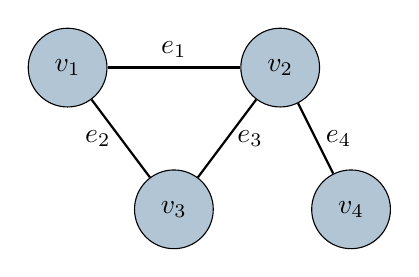
\begin{tikzpicture}[scale=0.9]
                    \node[draw, circle, fill=uibblue!30, minimum size=1cm] (A) at (0,2) {$v_1$};
                    \node[draw, circle, fill=uibblue!30, minimum size=1cm] (B) at (3,2) {$v_2$};
                    \node[draw, circle, fill=uibblue!30, minimum size=1cm] (C) at (1.5,0) {$v_3$};
                    \node[draw, circle, fill=uibblue!30, minimum size=1cm] (D) at (4,0) {$v_4$};
                    
                    \draw[thick] (A) -- (B) node[midway, above] {$e_1$};
                    \draw[thick] (A) -- (C) node[midway, left] {$e_2$};
                    \draw[thick] (B) -- (C) node[midway, right] {$e_3$};
                    \draw[thick] (B) -- (D) node[midway, right] {$e_4$};
                \end{tikzpicture}
            \end{center}
            
            \vspace{2mm}
            
            $V = \{v_1, v_2, v_3, v_4\}$ \\
            $E = \{e_1, e_2, e_3, e_4\}$
        \end{column}
    \end{columns}
    
\end{frame}

% ---------------------------------------------------------------------
% N02
% ---------------------------------------------------------------------
\begin{frame}{N02: Directed vs. undirected graph}
    
    \begin{columns}
        \begin{column}{0.48\textwidth}
            \textbf{\faArrowsAltH\ Undirected graph:}
            \begin{itemize}
                \item Edges have no direction
                \item $A - B$ means mutual connection
                \item Example: Patient Similarity Networks (PSN)
            \end{itemize}
            
            \begin{center}
                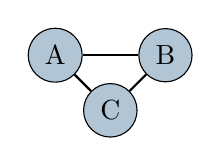
\begin{tikzpicture}[scale=0.7]
                    \node[draw, circle, fill=uibblue!30] (A) at (0,1) {A};
                    \node[draw, circle, fill=uibblue!30] (B) at (2,1) {B};
                    \node[draw, circle, fill=uibblue!30] (C) at (1,0) {C};
                    \draw[thick] (A) -- (B);
                    \draw[thick] (A) -- (C);
                    \draw[thick] (B) -- (C);
                \end{tikzpicture}
            \end{center}
        \end{column}
        
        \begin{column}{0.48\textwidth}
            \textbf{\faArrowRight\ Directed graph (digraph):}
            \begin{itemize}
                \item Edges have direction
                \item $A \rightarrow B \neq B \rightarrow A$
                \item Example: Gene regulatory networks
            \end{itemize}
            
            \begin{center}
                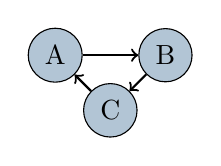
\begin{tikzpicture}[scale=0.7]
                    \node[draw, circle, fill=uibblue!30] (A) at (0,1) {A};
                    \node[draw, circle, fill=uibblue!30] (B) at (2,1) {B};
                    \node[draw, circle, fill=uibblue!30] (C) at (1,0) {C};
                    \draw[->, thick] (A) -- (B);
                    \draw[->, thick] (C) -- (A);
                    \draw[->, thick] (B) -- (C);
                \end{tikzpicture}
            \end{center}
        \end{column}
    \end{columns}
    
    \vspace{2mm}
    
    \begin{block}{\footnotesize \href{https://en.wikipedia.org/wiki/Directed_acyclic_graph}{Directed Acyclic Graph (DAG)}}
        \footnotesize A directed graph \textbf{without cycles} (no path $A \rightarrow \cdots \rightarrow A$). Used in causal inference, Bayesian networks, and workflow systems.
    \end{block}
    
    \vspace{1mm}
    
    \begin{block}{\footnotesize Medical context}
        \footnotesize PSN (patient similarity networks) are typically \textbf{undirected}: similarity between patient A and B is symmetric.
    \end{block}
    
\end{frame}

% ---------------------------------------------------------------------
% N03
% ---------------------------------------------------------------------
\begin{frame}{N03: Weighted vs. unweighted graph}
    
    \begin{columns}
        \begin{column}{0.48\textwidth}
            \textbf{Unweighted graph:}
            \begin{itemize}
                \item All edges are ``equal''
                \item Binary: connection or not
            \end{itemize}
            
            \begin{center}
                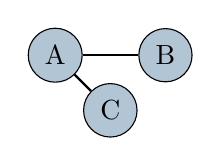
\begin{tikzpicture}[scale=0.7]
                    \node[draw, circle, fill=uibblue!30] (A) at (0,1) {A};
                    \node[draw, circle, fill=uibblue!30] (B) at (2,1) {B};
                    \node[draw, circle, fill=uibblue!30] (C) at (1,0) {C};
                    \draw[thick] (A) -- (B);
                    \draw[thick] (A) -- (C);
                \end{tikzpicture}
            \end{center}
        \end{column}
        
        \begin{column}{0.48\textwidth}
            \textbf{Weighted graph:}
            \begin{itemize}
                \item Edges have numerical weights
                \item Represents strength/distance/similarity
            \end{itemize}
            
            \begin{center}
                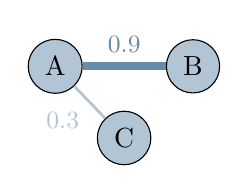
\begin{tikzpicture}[scale=0.7]
                    \node[draw, circle, fill=uibblue!30] (A) at (0,1) {A};
                    \node[draw, circle, fill=uibblue!30] (B) at (2.5,1) {B};
                    \node[draw, circle, fill=uibblue!30] (C) at (1.25,-0.3) {C};
                    \draw[thick, line width=3pt, uibblue!60] (A) -- (B) node[midway, above] {\small 0.9};
                    \draw[thick, line width=1pt, uibblue!30] (A) -- (C) node[midway, below left] {\small 0.3};
                \end{tikzpicture}
            \end{center}
        \end{column}
    \end{columns}
    
    \vspace{3mm}
    
    \begin{block}{In PSN (patient similarity networks)}
        \footnotesize
        The weight represents \textbf{similarity} between patients, calculated from clinical variables.\\[2pt]
        \textbf{Higher weight} ($w$) = more similar patients (similar symptoms, biomarkers, disease course, BMI, same gender, \ldots).\\
        \textbf{Lower weight} = less similar patients.\\
        Often a \textbf{threshold value} is used to filter out weak connections (e.g. $w < 0.5$).
    \end{block}
    
\end{frame}

% ---------------------------------------------------------------------
% N04
% ---------------------------------------------------------------------
\begin{frame}{N04: \href{https://en.wikipedia.org/wiki/Adjacency_matrix}{Adjacency Matrix}}
    
    \begin{columns}
        \begin{column}{0.4\textwidth}
            \begin{center}
                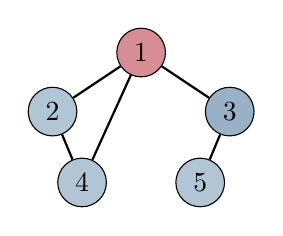
\begin{tikzpicture}[scale=0.75]
                    \node[draw, circle, fill=uibred!50] (1) at (1.5,2.2) {1};
                    \node[draw, circle, fill=uibblue!30] (2) at (0,1.2) {2};
                    \node[draw, circle, fill=uibblue!40] (3) at (3,1.2) {3};
                    \node[draw, circle, fill=uibblue!30] (4) at (0.5,0) {4};
                    \node[draw, circle, fill=uibblue!30] (5) at (2.5,0) {5};
                    
                    \draw[thick] (1) -- (2);
                    \draw[thick] (1) -- (3);
                    \draw[thick] (1) -- (4);
                    \draw[thick] (2) -- (4);
                    \draw[thick] (3) -- (5);
                \end{tikzpicture}
            \end{center}
            \scriptsize
            deg: 1$\rightarrow$3, 2$\rightarrow$2, 3$\rightarrow$2, 4$\rightarrow$2, 5$\rightarrow$1
        \end{column}
        
        \begin{column}{0.55\textwidth}
            \textbf{Adjacency Matrix $A$:}
            
            \[
            A = \begin{pmatrix}
            0 & 1 & 1 & 1 & 0 \\
            1 & 0 & 0 & 1 & 0 \\
            1 & 0 & 0 & 0 & 1 \\
            1 & 1 & 0 & 0 & 0 \\
            0 & 0 & 1 & 0 & 0
            \end{pmatrix}
            \]
            
            \begin{itemize}
                \item $A_{ij} = 1$ if edge between node $i$ and $j$
                \item $A_{ij} = 0$ otherwise
                \item Symmetric for undirected graphs
            \end{itemize}
        \end{column}
    \end{columns}
    
    \vspace{3mm}
    
    \begin{block}{Weighted graph}
        In weighted graph: $A_{ij} = w_{ij}$ (the weight of the edge)
    \end{block}
    
\end{frame}

% =====================================================================
\section{Centrality Measures}
% =====================================================================

% ---------------------------------------------------------------------
% N05
% ---------------------------------------------------------------------
\begin{frame}{N05: \href{https://en.wikipedia.org/wiki/Degree_centrality}{Degree Centrality}}
    
    \begin{columns}
        \begin{column}{0.5\textwidth}
            \begin{block}{Definition}
                \textbf{Degree} = number of edges to a node
                \[
                C_D(v) = \frac{\deg(v)}{n-1}
                \]
                (normalized: divided by max possible neighbors)
            \end{block}
            
            \vspace{2mm}
            
            \textbf{Interpretation:}
            \begin{itemize}
                \item High degree = many connections
                \item ``Hub'' in the network
                \item Easy to calculate
            \end{itemize}
        \end{column}
        
        \begin{column}{0.45\textwidth}
            \begin{center}
                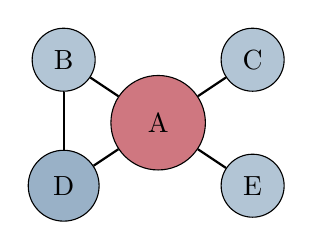
\begin{tikzpicture}[scale=0.8]
                    \node[draw, circle, fill=uibred!60, minimum size=1.2cm] (A) at (1.5,1.5) {A};
                    \node[draw, circle, fill=uibblue!30, minimum size=0.8cm] (B) at (0,2.5) {B};
                    \node[draw, circle, fill=uibblue!30, minimum size=0.8cm] (C) at (3,2.5) {C};
                    \node[draw, circle, fill=uibblue!40, minimum size=0.9cm] (D) at (0,0.5) {D};
                    \node[draw, circle, fill=uibblue!30, minimum size=0.8cm] (E) at (3,0.5) {E};
                    
                    \draw[thick] (A) -- (B);
                    \draw[thick] (A) -- (C);
                    \draw[thick] (A) -- (D);
                    \draw[thick] (A) -- (E);
                    \draw[thick] (D) -- (B);
                \end{tikzpicture}
            \end{center}
            
            \scriptsize
            \begin{tabular}{lcc}
            Node & deg & $C_D$ (norm.) \\
            \hline
            A & 4 & 1.00 \\
            B & 2 & 0.50 \\
            C & 1 & 0.25 \\
            D & 2 & 0.50 \\
            E & 1 & 0.25
            \end{tabular}
        \end{column}
    \end{columns}
    
    \vspace{1mm}
    
    \begin{block}{\footnotesize Medical relevance}
        \footnotesize In PSN: Patients with high degree centrality are similar to many others $\rightarrow$ ``typical'' patients.
    \end{block}
    
\end{frame}

% ---------------------------------------------------------------------
% N06
% ---------------------------------------------------------------------
\begin{frame}{N06: \href{https://en.wikipedia.org/wiki/Betweenness_centrality}{Betweenness Centrality}}
    
    \begin{columns}
        \begin{column}{0.5\textwidth}
            \begin{block}{Definition}
                Fraction of shortest paths that pass through a node
                \[
                C_B(v) = \sum_{s \neq v \neq t} \frac{\sigma_{st}(v)}{\sigma_{st}}
                \]
                $\sigma_{st}$ = number of shortest paths from $s$ to $t$
            \end{block}
            
            \vspace{2mm}
            
            \textbf{Interpretation:}
            \begin{itemize}
                \item High betweenness = ``bridge'' between groups
                \item Controls information flow
                \item Critical for network structure
            \end{itemize}
        \end{column}
        
        \begin{column}{0.45\textwidth}
            \begin{center}
                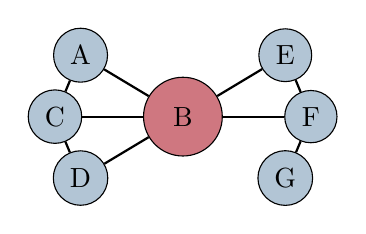
\begin{tikzpicture}[scale=0.65]
                    % Left cluster
                    \node[draw, circle, fill=uibblue!30] (A) at (0,2.2) {A};
                    \node[draw, circle, fill=uibblue!30] (C) at (-0.5,1) {C};
                    \node[draw, circle, fill=uibblue!30] (D) at (0,-0.2) {D};
                    
                    % Bridge
                    \node[draw, circle, fill=uibred!60, minimum size=1cm] (B) at (2,1) {B};
                    
                    % Right cluster
                    \node[draw, circle, fill=uibblue!30] (E) at (4,2.2) {E};
                    \node[draw, circle, fill=uibblue!30] (F) at (4.5,1) {F};
                    \node[draw, circle, fill=uibblue!30] (G) at (4,-0.2) {G};
                    
                    % Left cluster edges
                    \draw[thick] (A) -- (C);
                    \draw[thick] (C) -- (D);
                    % Bridge connections
                    \draw[thick] (A) -- (B);
                    \draw[thick] (C) -- (B);
                    \draw[thick] (D) -- (B);
                    % Right cluster edges
                    \draw[thick] (B) -- (E);
                    \draw[thick] (B) -- (F);
                    \draw[thick] (E) -- (F);
                    \draw[thick] (F) -- (G);
                \end{tikzpicture}
            \end{center}
            
            \scriptsize
            \begin{tabular}{cc|cc}
            Node & $C_B$ & Node & $C_B$ \\
            \hline
            A & 0.0 & E & 0.0 \\
            B & \textbf{15.0} & F & 2.0 \\
            C & 1.0 & G & 0.0 \\
            D & 0.0 & & 
            \end{tabular}
            
            \textit{Node B is bridge between two clusters}
        \end{column}
    \end{columns}
    
\end{frame}

% ---------------------------------------------------------------------
% N07
% ---------------------------------------------------------------------
\begin{frame}{N07: \href{https://en.wikipedia.org/wiki/Eigenvector_centrality}{Eigenvector Centrality}}
    
    \begin{block}{Idea}
        A node is important if it is connected to \textbf{other important nodes}
    \end{block}
    
    \vspace{2mm}
    
    \begin{columns}
        \begin{column}{0.55\textwidth}
            \textbf{Calculation:}
            \[
            x_i = \frac{1}{\lambda} \sum_{j \in N(i)} x_j
            \]
            
            Matrix form: $\mathbf{Ax} = \lambda \mathbf{x}$ (\href{https://en.wikipedia.org/wiki/Eigenvalues_and_eigenvectors}{eigenvector} equation)
            
            \vspace{2mm}
            
            \textbf{Difference from degree:}
            \begin{itemize}
                \item Degree: only counts number of neighbors
                \item Eigenvector: weights neighbors by their importance
            \end{itemize}
        \end{column}
        
        \begin{column}{0.4\textwidth}
            \begin{center}
                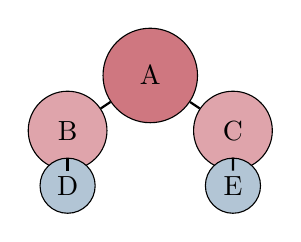
\begin{tikzpicture}[scale=0.7]
                    \node[draw, circle, fill=uibred!60, minimum size=1.2cm] (A) at (1.5,2) {A};
                    \node[draw, circle, fill=uibred!40, minimum size=1cm] (B) at (0,1) {B};
                    \node[draw, circle, fill=uibred!40, minimum size=1cm] (C) at (3,1) {C};
                    \node[draw, circle, fill=uibblue!30, minimum size=0.7cm] (D) at (0,0) {D};
                    \node[draw, circle, fill=uibblue!30, minimum size=0.7cm] (E) at (3,0) {E};
                    
                    \draw[thick] (A) -- (B);
                    \draw[thick] (A) -- (C);
                    \draw[thick] (B) -- (D);
                    \draw[thick] (C) -- (E);
                \end{tikzpicture}
            \end{center}
            
            \textit{A has highest eigenvector centrality}
        \end{column}
    \end{columns}
    
    \vspace{1mm}
    
    \begin{block}{\footnotesize Famous application}
        \footnotesize \href{https://en.wikipedia.org/wiki/PageRank}{Google PageRank} is a variant of eigenvector centrality!
    \end{block}
    
\end{frame}

% ---------------------------------------------------------------------
% N08
% ---------------------------------------------------------------------
\begin{frame}{N08: \href{https://en.wikipedia.org/wiki/Clustering_coefficient}{Clustering Coefficient}}
    
    \begin{block}{Definition}
        How much the neighbors of a node are connected to each other
        \[
        C_i = \frac{\text{number of edges between neighbors}}{\text{max possible edges between neighbors}}
        \]
    \end{block}
    
    \vspace{2mm}
    
    \begin{columns}
        \begin{column}{0.48\textwidth}
            \textbf{High clustering ($C = 1$):}
            \begin{center}
                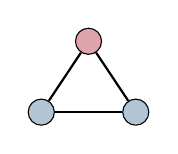
\begin{tikzpicture}[scale=0.6]
                    \node[draw, circle, fill=uibred!40] (A) at (1,2) {};
                    \node[draw, circle, fill=uibblue!30] (B) at (0,0.5) {};
                    \node[draw, circle, fill=uibblue!30] (C) at (2,0.5) {};
                    \draw[thick] (A) -- (B);
                    \draw[thick] (A) -- (C);
                    \draw[thick] (B) -- (C);
                \end{tikzpicture}
            \end{center}
            ``The neighbors know each other''
        \end{column}
        
        \begin{column}{0.48\textwidth}
            \textbf{Low clustering ($C = 0$):}
            \begin{center}
                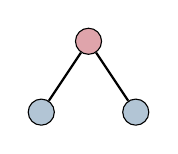
\begin{tikzpicture}[scale=0.6]
                    \node[draw, circle, fill=uibred!40] (A) at (1,2) {};
                    \node[draw, circle, fill=uibblue!30] (B) at (0,0.5) {};
                    \node[draw, circle, fill=uibblue!30] (C) at (2,0.5) {};
                    \draw[thick] (A) -- (B);
                    \draw[thick] (A) -- (C);
                    % No edge between B and C
                \end{tikzpicture}
            \end{center}
            ``The neighbors don't know each other''
        \end{column}
    \end{columns}
    
    \vspace{1mm}
    
    \begin{block}{\footnotesize Medical relevance}
        \footnotesize High clustering in PSN can indicate tight patient subgroups (phenotypes).
    \end{block}
    
\end{frame}

% =====================================================================
\section{Community Detection}
% =====================================================================

% ---------------------------------------------------------------------
% N09
% ---------------------------------------------------------------------
\begin{frame}{N09: \href{https://en.wikipedia.org/wiki/Community_structure}{Community Detection} and the \href{https://en.wikipedia.org/wiki/Louvain_method}{Louvain Algorithm}}
    
    \begin{block}{Community Detection}
        Identify \textbf{groups} (communities) of densely connected nodes
    \end{block}
    
    \vspace{2mm}
    
    \begin{columns}
        \begin{column}{0.5\textwidth}
            \textbf{The Louvain algorithm:}
            \begin{enumerate}
                \item Start: each node = own group
                \item Move nodes to neighbor groups that increase \textbf{modularity}
                \item Repeat until no improvement
                \item Aggregate and repeat hierarchically
            \end{enumerate}
            
            \vspace{2mm}
            
            \textbf{\href{https://en.wikipedia.org/wiki/Modularity_(networks)}{Modularity} $Q$:}
            \footnotesize
            \[
            Q = \frac{1}{2m}\sum_{ij}\left[A_{ij} - \frac{k_i k_j}{2m}\right]\delta(c_i, c_j)
            \]
            \scriptsize $i,j$=nodes, $A_{ij}$=adjacency matrix, $m$=edges, $k_i$=degree of node $i$, $c_i$=community of node $i$, $\delta$=1 if $c_i=c_j$. $Q > 0.3$: good structure.
        \end{column}
        
        \begin{column}{0.45\textwidth}
            \begin{center}
                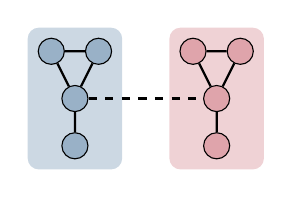
\begin{tikzpicture}[scale=0.6]
                    % Community 1
                    \fill[uibblue!20, rounded corners] (-0.5,-0.5) rectangle (1.5,2.5);
                    \node[draw, circle, fill=uibblue!40] (A) at (0,2) {};
                    \node[draw, circle, fill=uibblue!40] (B) at (1,2) {};
                    \node[draw, circle, fill=uibblue!40] (C) at (0.5,1) {};
                    \node[draw, circle, fill=uibblue!40] (D) at (0.5,0) {};
                    
                    % Community 2
                    \fill[uibred!20, rounded corners] (2.5,-0.5) rectangle (4.5,2.5);
                    \node[draw, circle, fill=uibred!40] (E) at (3,2) {};
                    \node[draw, circle, fill=uibred!40] (F) at (4,2) {};
                    \node[draw, circle, fill=uibred!40] (G) at (3.5,1) {};
                    \node[draw, circle, fill=uibred!40] (H) at (3.5,0) {};
                    
                    % Internal edges
                    \draw[thick] (A) -- (B) -- (C) -- (A);
                    \draw[thick] (C) -- (D);
                    \draw[thick] (E) -- (F) -- (G) -- (E);
                    \draw[thick] (G) -- (H);
                    
                    % Bridge edge
                    \draw[thick, dashed] (C) -- (G);
                \end{tikzpicture}
            \end{center}
            
            \textit{Two identified communities}
        \end{column}
    \end{columns}
    
\end{frame}

% ---------------------------------------------------------------------
% N10
% ---------------------------------------------------------------------
\begin{frame}{N10: The \href{https://networkx.org/}{NetworkX} library for Python}
    
    \begin{block}{NetworkX}
        Python library to create, manipulate, and analyze graphs
    \end{block}
    
    \vspace{2mm}
    
    \textbf{Common operations:}
    
    \begin{columns}
        \begin{column}{0.48\textwidth}
            \texttt{\small import networkx as nx} \\[2mm]
            \texttt{\small \# Create graph} \\
            \texttt{\small G = nx.Graph()} \\
            \texttt{\small G.add\_edge('A', 'B', weight=0.8)} \\
            \texttt{\small G.add\_edge('B', 'C', weight=0.5)} \\[2mm]
            \texttt{\small \# Centrality measures} \\
            \texttt{\small nx.degree\_centrality(G)} \\
            \texttt{\small nx.betweenness\_centrality(G)} \\
            \texttt{\small nx.eigenvector\_centrality(G)} \\
            \texttt{\small nx.clustering(G)}
        \end{column}
        
        \begin{column}{0.48\textwidth}
            \texttt{\small \# Community detection} \\
            \texttt{\small from community import louvain} \\
            \texttt{\small partition = louvain.best\_partition(G)} \\[2mm]
            \texttt{\small \# Visualization} \\
            \texttt{\small nx.draw(G, with\_labels=True)} \\[2mm]
            \texttt{\small \# From adjacency matrix (numpy)} \\
            \texttt{\small G = nx.from\_numpy\_array(A)} \\[2mm]
            \texttt{\small \# Graph properties} \\
            \texttt{\small G.number\_of\_nodes()} \\
            \texttt{\small G.number\_of\_edges()} \\
            \texttt{\small nx.density(G)}
        \end{column}
    \end{columns}
    
\end{frame}

% ---------------------------------------------------------------------
% Summary
% ---------------------------------------------------------------------
\begin{frame}{Summary: N01--N10}
    
    \begin{columns}
        \begin{column}{0.48\textwidth}
            \textbf{Graph theory fundamentals:}
            \begin{itemize}
                \item Graph $G = (V, E)$: nodes ($V$) + edges ($E$)
                \item Directed vs. undirected
                \item Weighted vs. unweighted
                \item Adjacency matrix representation
            \end{itemize}
            
            \vspace{3mm}
            
            \textbf{Centrality measures:}
            \begin{itemize}
                \item Degree: number of connections
                \item Betweenness: bridge role
                \item Eigenvector: important neighbors
            \end{itemize}
        \end{column}
        
        \begin{column}{0.48\textwidth}
            \textbf{Structural analysis:}
            \begin{itemize}
                \item Clustering coefficient: local density
                \item Community detection: finding groups
                \item Louvain algorithm: efficient method
            \end{itemize}
            
            \vspace{3mm}
            
            \textbf{Tools:}
            \begin{itemize}
                \item \href{https://networkx.org/}{NetworkX} (Python)
                \item Integration with \href{https://numpy.org/}{NumPy}/\href{https://pandas.pydata.org/}{Pandas}
            \end{itemize}
        \end{column}
    \end{columns}
    
    \vspace{5mm}
    
    \begin{block}{Next steps}
        Use these concepts to build \textbf{patient similarity networks} (PSN)!
    \end{block}
    
\end{frame}

\end{document}
